\label{sec:twa}

\newcommand{\dfs}{search\xspace}
In this chapter we discuss a less standard automaton model for finite trees -- as opposed to tree automata discussed in Chapter~\ref{sec:tree-aut} -- namely tree-walking automata. We show  that tree-walking automata cannot be not determinised.

The point of a tree-walking automaton is to have a run that is  sequential, i.e.~it  is a sequence -- and not a tree -- of configurations. The idea is that at any  moment of its run, the automaton is in a single node of the input tree. Based on the local view, which is this information 
\mypicb{93}
and the current state,  
 the automaton chooses the new state and a neighbour (possibly  the parent) to move to, or to accept or reject. The information on the child number is useful for operations like depth-first search, and the model becomes powerless if the child number is not included in the local view, see the exercises. 

\begin{definition}[Tree-walking automaton]
The syntax of a  \emph{(nondeterministic) tree-walking automaton} consists of: a finite ranked set $\Sigma$ called the \emph{input alphabet}, a finite set of states $Q$ with designated initial and accepting subsets, and a transition relation of the form 
\mypicb{94}
		We assume that for every transition, the local view (i.e.~the second coordinate) is consistent with the direction of the move (i.e.~the last coordinate)  in the sense that if the direction  is ``parent'' then local view says that there is a parent,  and if the direction is ``child $i$'' then local view says that there is an $i$-th child.
The automaton is called \emph{deterministic} if it has one initial state and  the  transition relation is  a function from the first two arguments to the last two arguments.
\end{definition}

 Consider an input tree over the input alphabet. A \emph{configuration} of the automaton is a pair (state, node of the input tree).   A run of the automaton is a sequence of configurations, such that every two consecutive configurations are connected by the transition relation in the natural way, illustrated in the following picture: \mypicb{88}
The automaton accepts a tree if there is a run which begins in an  initial state at the root of the tree, and which ends in a configuration that uses an accepting state.  For a deterministic tree-walking automaton,  there are two ways of rejecting an input tree: (a) reaching a configuration that  has no applicable transition; (b) entering an infinite loop. Using a construction from~\cite[Theorem 1]{Sipser:1980fp}, one can show that every deterministic tree-walking automaton can be modified so that rejection is done only via (a), see~\cite[Proposition 1]{Muscholl:2006cl}.


\begin{example}\label{ex:dfs}
Consider the following ranked alphabet 
\mypicb{42}
The tree language ``at least one black leaf'' can be recognised by a nondeterministic tree-walking automaton, which uses nondeterminism to find the black leaf. If we want to avoid nondeterminism, or we want to recognise the language ``all leaves are white'', then  we can use an automaton that does a depth-first search through the tree. This automaton has three states: 
\mypicb{30}
which stand, respectively, for the first, second and third visit to a node. The   transition relation is defined so that the run looks like in the following picture:
\mypicb{91}
\end{example}

\section{Tree-walking automata cannot be determinised}
The goal of this chapter is to prove that tree-waking automata cannot be determinised. 
\begin{theorem}\label{thm:twa-det}\cite[Theorem 5]{Bojanczyk:2006ff}
	There is a tree language that is recognised by a nondeterministic tree-walking automaton, but not by any deterministic tree-walking automaton.
\end{theorem}
In the exercises, we show that nondeterministic tree-walking automata can be converted into  tree automata as defined in Chapter~\ref{sec:tree-aut}. The converse does not hold, i.e.~there is a language recognised by a tree automaton that is not recognised by any (nondeterministic) tree-walking automaton~\cite[Theorem 2]{Bojanczyk:2008cx}. 

The rest of this chapter is devoted to proving Theorem~\ref{thm:twa-det}.
We begin by defining the language which separates deterministic and nondeterministic tree-walking automata, and we show that the language can be recognised by a nondeterministic tree-walking automaton. In the next section we show the lower bound --  the separating language cannot be recognised by a deterministic automaton.

\paragraph*{The separating language.} 
The input alphabet for the separating language is the same as in Example~\ref{ex:dfs}, i.e.~there is a binary white letter and  two leaf letters in the colours white and black. 
The language consists of trees with exactly three black leaves, such that  the  black leaves are distributed  \mypicb{43}
\begin{lemma}\label{lem:ntwa}
The separating language is recognised by a nondeterministic tree-walking automaton.
\end{lemma}
\begin{proof}
The automaton first does a depth-first search, as explained in Example~\ref{ex:dfs}, to check if the tree contains exactly three black nodes. If not, it rejects. Otherwise, it uses a depth-first search to return to the first black node, and then it uses nondeterminism to go to some  ancestor $v$ of the first black node. The  idea is that $v$  will be chosen as in the following picture:
\mypicb{39}
Next, the automaton continues a depth-first search, as if it has just visited $v$ for the third time: \mypicb{95}
The automaton accepts if during the remainder of  this depth-first search, it sees exactly  one black node.  If the input tree belongs to the language,  then by choosing $v$ as in (*), the automaton will accept. If the input tree is outside the language, i.e.~the shape is like this: \mypicb{38}
 then no matter how $v$ is chosen, the automaton will see either zero or two black leaves in its depth-first search after visiting $v$. Therefore the automaton accepts all trees in the separating language, and no other trees.
\end{proof}

\paragraph*{The lower bound.}
We now turn to the heart of Theorem~\ref{thm:twa-det}, i.e.~showing that a deterministic tree-walking automaton cannot recognise the separating language. We will show that  for specially crafted  inputs, a deterministic tree-walking automaton can only do a depth-first search, and this is not enough to recognise the separating language. Fix for the rest of this section a deterministic tree-walking automaton. We will prove that this automaton does not recognise the separating language. From now on, when talking about local views, we talk about local views for the alphabet in the separating example.

\paragraph*{Patterns.} A \emph{pattern} is defined similarly to a tree (over our fixed input alphabet), with the exception that a subset of nodes --  called \emph{ports} -- is  labelled by local views instead of letters from the input alphabet,  subject to constraints (A), (B), (C) in the picture below (the ports are the nodes that are not on a blue background):
\mypicb{40}
A pattern without any ports is the same  as a tree.  Define the \emph{arity} of a pattern to be the number of leaf ports. 

Patterns are composed as follows. Let $t$ be an $n$-ary pattern and let  $t_1,\ldots,t_n$ be patterns such that for every  $i \in \set{1,\ldots,n}$, the root of pattern $t_i$  is a port which  has the  same local view as the $i$-th leaf port in $t$. Then their composition is defined by fusing the corresponding ports -- the $i$-th leaf port of $t$ with the root port of $t_i$ --  as in the following picture:
\mypicb{16}

\paragraph*{Equivalence.} To show that our fixed deterministic tree-walking automaton cannot recognise the separating language,  we will find two patterns that are equivalent with respect to the automaton, but which are not equivalent with respect to the language. Define a \emph{port-to-port} run  inside a pattern  to be a sequence of configurations as depicted in the following picture
\mypicb{96}
 The \emph{type} of a port-to-port run  is defined to be the following information: (a) what is the state and port in the source configuration (b) what is the state and port in the target configuration (or accept / reject / loop if the run does not reach any port).  In the type, we do not store the actual port node, only its number (i.e.~is it the root port, leaf port 1, leaf port 2, etc.). In particular, the number of types of runs is finite once the arity of a pattern is fixed. Two patterns are called \emph{equivalent} if: they have the same local view in the root (or the root is not a port in both patterns), they have the same number of leaf ports with the same respective local views, and they have  the same types of port-to-port runs. Pattern equivalence  is a congruence, i.e.~composing equivalent patterns gives equivalent results.
 
\newcommand{\locview}{\includegraphics[page=22,scale=0.3]{picsb}\xspace}

We now move to the first main ingredient in the proof.  If $T$ is a set of patterns, then we write $T^+$ for the least set of patterns that contains $T$ and is closed under pattern composition.
\begin{lemma}\label{lem:patterns}[Homogeneous Pattern Lemma]
	There exist patterns $t_0,t_1,t_2$ with the following properties:
	\begin{enumerate}
		\item For every $i \in \set{0,1,2}$, $t_i$  does not have black nodes,   has a root port and $i$ leaf ports, and has the local view \locview in all ports.
		\item For every $i \in \set{0,1,2}$, all $i$-ary patterns in $\set{t_0,t_1,t_2}^+$  are equivalent.
	\end{enumerate}
\end{lemma}
We draw the patterns from the lemma like this:
\mypicb{17}
with the white circles standing for ports. The point of all ports having the same local view \locview is that the patterns can be freely composed.
We use the name \emph{homogeneous pattern} for patterns in  $\set{t_0,t_1,t_2}^+$. In this terminology, item 2 of the lemma says that all homogeneous patterns of fixed arity $i \in \set{0,1,2}$ are equivalent. 
For example, all of the following homogeneous binary patterns are equivalent, because they have arity 2 (we adopt the convention that ports are drawn as white, and ports connecting patterns are drawn in colours like yellow or red, although they represent nodes with  local view \locview):
\mypicb{18} 
When proving the Homogeneous Pattern Lemma, we use the following result about finite semigroups. Recall that a semigroup is a set with an associative product operation.
\begin{lemma}[Semigroup Lemma]
Let $S$ be a finite semigroup with elements $a,b$. There exist elements $x \in aS$ and $y \in bS$ which satisfy 
\begin{align*}
x = xx = xy.
\end{align*}
\end{lemma}
\begin{proof} The key result is the following well-known observation on finite semigroups: there is an \emph{idempotent power}, i.e.~a number $\omega \in \set{1,2,\ldots}$ such that every element satisfies $s^\omega = s^\omega s^\omega$. 
More specifically, we take $\omega$ to be the factorial of the size of the semigroup. We now show that
\begin{align*}
  s^\omega = s^\omega s^\omega \qquad \text{for every }s \in S.
\end{align*}
Let then $s \in S$. By considering the first repetition in the sequence $s^1, s^2,\ldots$ we see that there exist numbers $i,j $, which  are at most the size of the semigroup, and such that $s^i = s^{i+1}$.
Because $i \le \omega$ and $j$ divides $\omega$, we get
\begin{align*}
  s^{\omega} = s^{\omega+j} = s^{\omega+2j} = \cdots = s^{\omega + \omega} = s^{\omega}s^{\omega},
\end{align*}
thus proving that $\omega$ is an idempotent power. To prove the lemma,  define
\begin{align*}
  y \eqdef b^{\omega}  \qquad x \eqdef  (ay)^{\omega}
\end{align*}
In particular, both $x$ and $y$ are idempotents, because each is obtained by taking some element to the idempotent power. This establishes $x = xx$. Furthermore, since $x$ ends with the idempotent $y$, we get $x = xy$.
\end{proof}


\begin{proof}[Proof of the Homogeneous Patterns Lemma] For $n \in \set{1,2,\ldots}$, define $s_n$ to be the pattern depicted in the following picture:
\mypicb{27}
Because equivalence on patterns has finitely many equivalence classes, there must be some numbers $n < N$ such that $s_n$ and $s_N$ are equivalent.   Define $t_0$, the first of the homogeneous patterns from the statement of the lemma, to be $s_n$. 

Choose distinct nodes  in the pattern $s_N$ which are right children  and  have subtrees of depth $n$. 
Define $s$ to be the binary  pattern obtained from $s_N$ by putting a leaf port in each of these chosen nodes, here is a picture of $s$ for $n=2$ and $N=4$:
\mypicb{33}
For the rest of the proof, we will draw the patterns $t_0$ and $s$ like this:
\mypicb{20}
By definition, $s[t_0,t_0]=s_N$, which is equivalent to $s_n=t_0$. By induction, this generalises to the fact that  all rank $0$ patterns in $\set{s,t_0}^+$ are equivalent. 

In the following claim, we use multiplicative notation for composition of unary patterns.

\begin{claim}\label{claim:twa1}
	There are unary patterns $A,B \in \set{s,t_0}^+$ such that $
  x = xx = xy$  holds for 
 \mypicb{90}
\end{claim}
\begin{proof}
Apply the Semigroup Lemma to the  semigroup of unary patterns (modulo pattern equivalence)  generated by the following patterns:
\mypicb{23}
\end{proof}

Let $A,B$ and $x,y$ be as in the above claim. Define $t_1$ to be $x$ and define
\mypicb{32}
This completes the definition of the patterns $t_0,t_1,t_2$. 
From the claim, we get the following equivalence: 
\mypicb{21}
A symmetric proof also gives the following equivalence:
\mypicb{31}
Directly from the claim, $t_1$ is idempotent in the following sense
\mypicb{24}
Since $t_2$ has $t_1$  attached to  each of its ports,  idempotence of $t_1$ implies that:
 \mypicb{25}
Because $t_1$ is from $\set{s,t_0}^+$, we get that
\mypicb{26}
 Using the above equivalences, and induction on the size of a pattern, one shows that every homogeneous patterns of arity $i \in \set{0,1,2}$ is equivalent to $t_i$.
\end{proof}
The  Homogeneous  Pattern Lemma would also work for nondeterministic tree-walking automata, and even tree automata as in Chapter~\ref{sec:tree-aut} ones under a suitable notion of equivalence. In contrast, the following lemma crucially depends on determinism (actually, a stronger result is true, namely every two homogeneous patterns of same arity are equivalent, see Exercise~\ref{zad:tree-aut-04}).
\begin{lemma}[Rotation Lemma]
The following two patterns are equivalent:
\mypicb{19}
\end{lemma}

The lemma immediately implies the lower bound from Theorem~\ref{thm:twa-det}, i.e.~that a deterministic tree-walking automaton cannot recognise the separating language, thus finishing the proof of Theorem~\ref{thm:twa-det}. Indeed,  take the two patterns in the Rotation Lemma, and put them into the following environment:
\mypicb{87}
The tree on the left should be accepted and the tree on the right should be rejected, but the automaton will behave the same way on both trees by the Rotation Lemma. It remains to prove the Rotation Lemma.

\section{Proof of the rotation lemma}
\label{sec:rotation-lemma}
In this section, we prove the Rotation Lemma. The proof uses a detailed analysis of what a deterministic tree-walking automaton can do in a homogeneous pattern. The bottom line is that the most interesting behaviour that it can do is a depth-first search.
\paragraph*{Closure of a state.} 
For a state $q$, consider the run of the automaton which begins in state $q$ in the yellow node below:
\mypicb{83}
and which is cut off at the first visit  to a port node (white in the picture).
Define the \emph{closure} of $q$, denoted by $\bar q$, to be the following information:
\begin{itemize}
	\item \emph{if the run reaches a port}: the state of the last visit in the yellow node;
	\item \emph{if the run does not reach a port}: does it accept / reject / loop.
\end{itemize}
We might have $q = \bar q$ if the run goes directly to from the yellow node to some port, without every seeing the yellow node again.
The definition of closure is based on the behaviour of the automaton on the interface between two copies of $t_1$. The following lemma shows that the same behaviour will be witnessed on the interface between any two homogeneous patterns of nonzero arity.
\begin{lemma}\label{lem:twa-bar}
  Let $s,t$ be homogeneous patterns of nonzero arity, and let $i$ be one of the leaf ports in $s$. If the automaton begins in state $q$ in the yellow node here: \mypicb{84}
  then:  (a) if $\bar q$ is one of  accept / reject / loop  then the automaton will do the same without reaching any ports; and (b)
  if $\bar q$ is a state then the automaton will visit the yellow node for the last time in state $q$ and then go to some port. \end{lemma}
\begin{proof} 
Case (a) is illustrated in the following picture
\mypicb{85}
For case (b), suppose  that $\bar q$ is a state. Consider the following run \mypicb{86}
Item (1) above is by the definition of $\bar q$  applied to the part of the pattern between the red nodes. Item (2) above is by the definition of $\bar q$  applied to the entire pattern. 
Consider now the port-to-port run which starts in the yellow node of the pattern from case (a). By item (1), the yellow node will be visited in state $\bar q$ before any  of the ports are visited. By item (2), the last visit in the yellow node will be in port $\bar q$, and then one of the ports will be visited.
\end{proof}





\begin{lemma}\label{lem:closure-up} For every states $p,q$ we have the following implications (and their symmetric versions with leaf port 2 used instead of leaf port 1):
  \mypicb{60}
\end{lemma}
\begin{proof}
We only prove the first implication, the other ones are proved the same way.
Consider the following port-to-port run:
\mypicb{37}
Item (1) in the picture is  the assumption of the implication. Item (2) is by definition of $\bar q$ and Lemma~\ref{lem:twa-bar}. Item (3) is again the assumption of the implication applied to the entire pattern. The run from (2) to (3) witnesses the conclusion of the implication. \end{proof}

\paragraph*{Search behaviour.} We now turn to the crucial definition in the proof of the Rotation Lemma. 

\begin{definition}
We say that a state $q$ is a left-to-right \dfs if there exists some state $p$ such  that the automaton admits the following port-to-port runs:
	\mypicb{53}
\end{definition}
The following straightforward lemma shows that a left-to-right \dfs will visit leaf ports in left-to-right order.
\begin{lemma}\label{lem:dfs-does}
Assume that a state $q$ is a left-to-right \dfs. Then:
\begin{itemize}
	\item[(*)]if  the automaton enters a homogeneous $n$-ary pattern in state $\bar q$ at  leaf port $i<n$, then it will exit through the next leaf port $i+1$.
\end{itemize}
\end{lemma}
\begin{proof}
Here is the run that witnesses (*).
\mypicb{44}
In the picture above, we use Lemma~\ref{lem:twa-bar} to prove that if a node is first visited in state $q$, then it is last visited in state $\bar q$, likewise for $p$. 
\end{proof}
We now state the most technical part of the proof, which says that the conclusion (*) above is also true for any state $r$ which goes from leaf port 1 to leaf port 2 in the pattern $t_2$.

\begin{lemma}\label{lem:get-dfs}
Suppose $r,p$ are states which admit the following port-to-port run:
\mypicb{45}
Then the conclusion (*) of Lemma~\ref{lem:dfs-does} is true with $r$ used instead of $\bar q$.
\end{lemma}
\begin{proof}
We claim that there  is a state $q$ which is a left-to-right \dfs and satisfies 
\mypicb{63}
Before proving the claim, we use it to prove the lemma. Let  $t$ be an $n$-ary homogeneous pattern and let $i < n$ be one of the root ports. The following picture shows the run that witnesses (*) in the conclusion of the lemma. \mypicb{74}
Item (1) is by ($\uparrow$) and Lemma~\ref{lem:twa-bar}, and item (2) is from Lemma~\ref{lem:dfs-does}. 

The rest of the proof is devoted to proving the claim, i.e.~finding a state $q$ which satisfies ($\uparrow$) and is a left-to-right search. Consider the following port-to-port  run, which exists by the assumption of the lemma:
\mypicb{79}
The red node must be  visited by the above run, since it is on the way from leaf port 1 to leaf port 2. We first claim that in the run above, the yellow node cannot be visited. Otherwise, part of the run would look like this 
\mypicb{59}
Items (3) and (4) are by Lemma~\ref{lem:closure-up} applied to the part of the run between (1) and (2). Item (4)  contradicts the assumption that the first port visited by the run in  ($\clubsuit$) is leaf port 2.   

Therefore, the run from ($\clubsuit$) never visits the yellow node. 
Define $q$ to be the state of the first visit in the red node. Because the red node is visited first, we have \mypicb{64}
	The conclusion above is ($\uparrow$) from the claim at the beginning of the proof. It remains to prove that $q$ is a left-to-right search. 
	Applying Lemma~\ref{lem:closure-up} to the leftmost picture above, we get 
	\mypicb{80}
The last time the red node is visited in the run from ($\clubsuit$) is in state $\bar q$. After this visit, the run goes to leaf port 2 in state $p$, thus proving 
	\mypicb{81} 
To complete the proof that $q$ is a left-to-right search, it remains to show: 
\mypicb{82}
Consider the port-to-port run described in the following picture:
\mypicb{70}

\begin{claim}
The red node is not visited between configurations (2) and (3).
\end{claim}
The claim establishes (***), which was the last ingredient required to show that state $q$ is a left-to-right search. It remains to show the claim  (actually, a finer analysis would show that the red node is not visited at all during the run.)  
\begin{proof}
Toward a contradiction, suppose that the red node is visited between configurations (2) and (3). Let $x$ be the state of the last visit to the red node. Then the automaton would have a run like this:
\mypicb{98}
The run from (2) to (i)  is taken from the assumption on $x$. The run from (i) to (ii)  is because the run in ($\clubsuit$) goes from the red node to leaf port 2 in state $p$. In particular, the run from (i) to (ii) implies that 
\mypicb{97}
which in turn yields the run from  (ii) to (iii). The run from (1) to (iii) shows 
\mypicb{99}
 which  contradicts  (**).
\end{proof}
\end{proof}
 
 
 \begin{proof}[Proof of the Rotation Lemma] 

To prove the Rotation Lemma, let  $\rho,\rho'$ be  port-to-port runs in the two patterns 
\mypicb{19}
from the statement of the Rotation Lemma, respectively, which have equivalent source configurations. To prove equivalence, we need to show that  target configurations are equivalent. Let $q$ be the state in the source configuration of the two runs. We consider two cases depending on the source port.
	\begin{enumerate}
		\item \emph{The runs begin in a leaf port.} The cases of leaf port 1 and 3 are symmetric, see we ignore the case of leaf port 3. Suppose that the automaton starts in leaf port 1 or 2. Let us see what happens in the pattern $t_2$ if we start in leaf port 1 in state $q$. There are three cases to consider:
	\mypicb{76}
	 In the first case, we use Lemma~\ref{lem:closure-up} to show that both $\rho$ and $\rho'$ end in the root port (and in the same state).
	 In the second case, we use Lemma~\ref{lem:dfs-does} to show that both $\rho$ and $\rho'$ end in leaf port $i+1$ (and in the same state).
 In the third case, we conclude that for every homogeneous pattern, if the automaton begins in state $q$ in a leaf port, then it will return to the same port (in some fixed state) or never visit any other ports (and have the same behaviour among accept / reject / loop). Here is the picture:
\mypicb{77}


	\item \emph{The runs begin in the root port.}  	Consider three cases for what happens if the automaton starts in the roof of $t_2$  in state $q$:
	\mypicb{35}
	For the first  case, we use  Lemma~\ref{lem:closure-up} to prove that both $\rho$ and $\rho'$ will end in leaf port 1. A symmetric reasoning is applied in the second case, with the target being leaf port 3. The third case is dealt with the same way as in the previous item.
		\end{enumerate}	

\end{proof}

